%%
%% This is file `mcmthesis-demo.tex',
%% generated with the docstrip utility.
%%
%% The original source files were:
%%
%% mcmthesis.dtx  (with options: `demo')
%% 
%% -----------------------------------
%% 
%% This is a generated file.
%% 
%% Copyright (C)
%%     2010 -- 2015 by Zhaoli Wang
%%     2014 -- 2015 by Liam Huang
%% 
%% This work may be distributed and/or modified under the
%% conditions of the LaTeX Project Public License, either version 1.3
%% of this license or (at your option) any later version.
%% The latest version of this license is in
%%   http://www.latex-project.org/lppl.txt
%% and version 1.3 or later is part of all distributions of LaTeX
%% version 2005/12/01 or later.
%% 
%% This work has the LPPL maintenance status `maintained'.
%% 
%% The Current Maintainer of this work is Liam Huang.

%% 
\documentclass{mcmthesis}
\mcmsetup{tcn = 233666, problem = B,
sheet = true, titleinsheet = true, keywordsinsheet = true,
titlepage = true, abstract = true}
\usepackage{palatino}
\usepackage{mwe}
\usepackage{amsmath}
\usepackage{indentfirst}
\usepackage{graphicx}
\usepackage{subfigure}
\usepackage{caption}
\setlength{\parindent} {2em}
\title{Sudoku Analyzing}
\author{Kai Feng, Song Lu, Yutao Zeng }
\date{\today}
\begin{document}
\begin{abstract}
here is the abstract!~!!
\begin{keywords}
keyword1; keyword2
\end{keywords}
\end{abstract}
\maketitle

\section{Introduction}
\subsection{Statement of Problem}
We set out to design an algorithm that would construct unique sudoku puzzles of various difficulties as well as to develop metrics by which to measure the difficulty of a given puzzle. In particular, our algorithm must admit at least four levels of difficulty while minimizing its level of complexity.

\subsection{Significance of Sudoku Research}
Sudoku is one of the most pupular puzzle games of all time, which is famous for its simple rules and puzzle diversity. We think that this problem is insteresting and of great significance, due to its inherently mathematical, and offers us an oppotunity to explore new mathematical techniques. After studying, we found out that this problem could be regarded as a derivation of the Latin Square puzzle, and can be solved by using the exact-cover method.\\
\indent Meanwhile, both solving and building the Sudoku puzzles are proved to be NP-Complete problems, which means that there is no known efficient way to locate an exact solution in the first place. It is apparently a great challenge for us to solve the problem in the polymonial time right now. But if we can make some progress,we may also expand into other and more practical problems. However, we shall restrict our focus directly to the problem at hand, and be content to leave these reasons, along with sudoku's entertainment value, as our motivation for exploring the game. 

\subsection{Sudoku Introduction}
Sudoku, is a logic-based,combinatorial number-placement puzzle. The objextive is to fill a $9\times9$ grid with digits so that each column, each row, and each of the nine $3\times3$ subgrids that compose the grid contains all of the digits from 1 to 9. The puzzle setter provides a partially completed grid, which for a well-posed puzzle has a unique solution. Figure.1(a) is a typical example of sudoku puzzle.

\begin{figure}[htbp]
\centering %居中
\subfigure[Typical sudoku puzzle]{ %第一张子图
\begin{minipage}{7cm}
\centering %子图居中
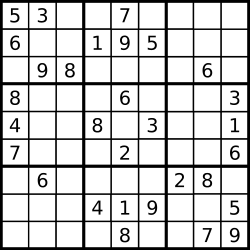
\includegraphics[scale=0.6]{figures/sudoku.png} %以pic.jpg的0.5倍大小输出
\end{minipage}
}
\subfigure[The same puzzle with solution]{ %第二张子图
\begin{minipage}{7cm}
\centering %子图居中
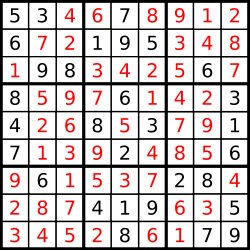
\includegraphics[scale=0.6]{figures/sudoku_complete.png} %以pic.jpg的0.5倍大小输出
\end{minipage}
}
\caption{sudoku puzzle instance} % %大图名称
\label{fig:1.3.1} %图片引用标记
\end{figure}

% \begin{figure}[htbp]
% \small
% \centering
% 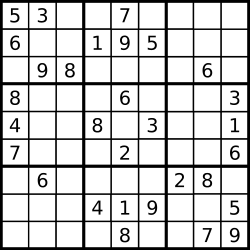
\includegraphics[width=6cm]{figures/sudoku.png}
% \caption{Typical sudoku puzzle} \label{fig:1.1}
% \end{figure}

\indent Completed games are always a type of Latin square with an additional constraint on the contents of individual regions. For example, the same single integer may not appear twice in the same row, column, or any of the nine $3\times3$ subregions of the $9\times9$ playing board.\newline

% \centerline{
% 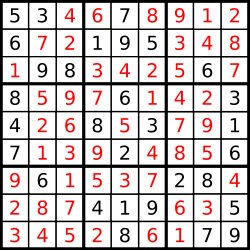
\includegraphics[width = 6cm]{figures/sudoku_complete.png}
% }
% \centerline{Fig.2 }

\subsection{Notations and Terminologies}
It is difficult to discuss our solution to the proposed problem without understanding some common
terminology. Moreover, since we will apply more mathematical formalism here than in most documents dealing with sudoku, it will be helpful to introduce notational conventions.

\begin{itemize}
	\item \textbf{Cell.} The basic unit of Sudoku puzzle. A square in the grid which may contain one digit(1-9). The grid is composed of 81 cells.

	\item \textbf{Block.} A $3\times3$ array of cells. Normally, the boundaries of the blocks are marked by slightly darker or thicker lines than the lines separating the cells. The grid is composed of 9 non-overlapping blocks. Each block must contain all the digits(form 1 to 9) and may not contain more than one of each digit.

	\item \textbf{Column.} A verticle line of 9 cells. The grid is composed of 9 columns. Each column must contain all the digits(1-9) and may not contain more than one of each digit.

	\item \textbf{Row.} A horizontal line of 9 cells. The grid is composed of 9 rows. Each row must contain all the digits (1-9) and may not contain more than one of each digit.

	\item \textbf{Grid.} The $9\times9$ array of cells that compose a Sudoku puzzle. The grid contains 9 rows, 9 columns and 9 blocks.

	\item \textbf{Puzzle.} A $9\times9$ matrix of cells, with at least one empty and at least one filled cell. For our purposes, we impose the additional requirement that all puzzles have exactly one solution. 	

	\item \textbf{House.} The column, row and block are collectively called the House.

	\item \textbf{Peer.} If two cells are in the same house (same row, same column, or same block) they are said to see each other, or to be peers.


	\item \textbf{Candidate.} Any digit that may be placed in an empty cell based on current state of the puzzle. If a digit is present in one or more of a cell's buddies, it cannot be a candidate for that cell. Analysis may further reduce the candidate set to a signle candidate, that candidate must be the sulution for that cell.

	\item \textbf{Analysis.} Any technique that eliminates candidates. Techniques of analysis do ultimately lead to solutions for cells, but it may take the application of multiple techniques or multiple applications of the same technique to reach a solution for a single cell. The point of analysis then, is to eliminate candidates, not look for solutions. Looking for solutions is scanning.
\end{itemize}

\subsection{Common Solving Strategy}
\subsubsection{Full House/Last Digit}
A Full House is simply the last digit that can be placed in a row,column or block. If it is the last digit for the whole grid, it is sometimes called "Last Digit".

\begin{figure}[ht]
\small
\centering
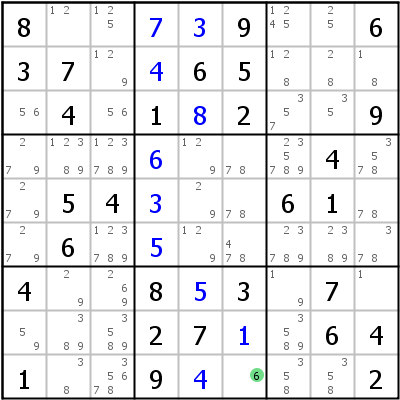
\includegraphics[width=7cm]{figures/full_house.png}
\caption{an example of full house} \label{fig:1.5.1}
\end{figure}

\subsubsection{Naked Single}
Naked Single means that in a specific cell only one digit remains possible (the last remaining candidate has no other candidates to hide behind and is thus naked). The digit must then go into that cell.

% \begin{figure}[ht]
% \small
% \centering
% 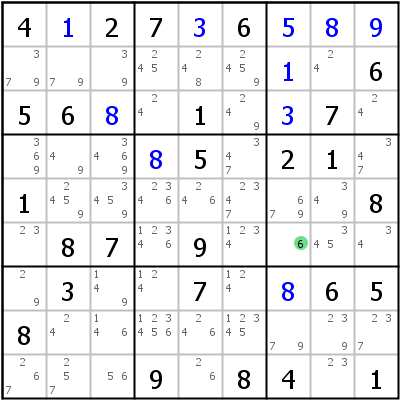
\includegraphics[width=5cm]{figures/naked_single.png}
% \caption{an example of naked single} \label{fig:02}
% \end{figure}

% \begin{figure}[ht]
% \small
% \centering
% 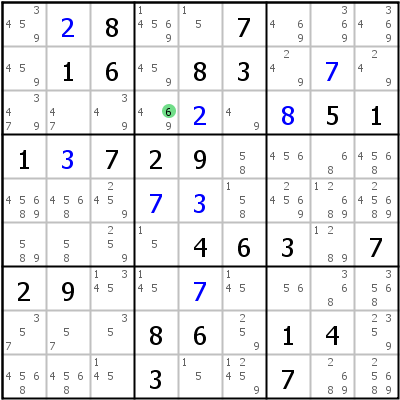
\includegraphics[width=5cm]{figures/hidden_single.png}
% \caption{an example of hidden single} \label{fig:03}
% \end{figure}

\begin{figure}[htbp]
\centering %居中
\subfigure[Naked Single]{ %第一张子图
\begin{minipage}{7cm}
\centering %子图居中
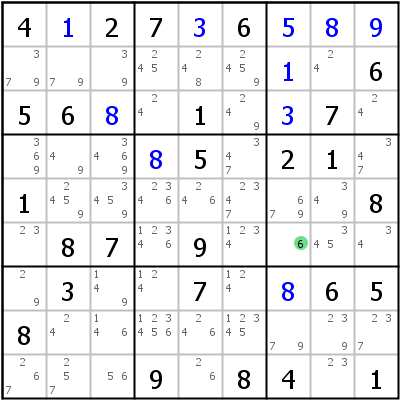
\includegraphics[scale=0.65]{figures/naked_single.png} %以pic.jpg的0.5倍大小输出
\end{minipage}
}
\subfigure[Hidden Single]{ %第二张子图
\begin{minipage}{7cm}
\centering %子图居中
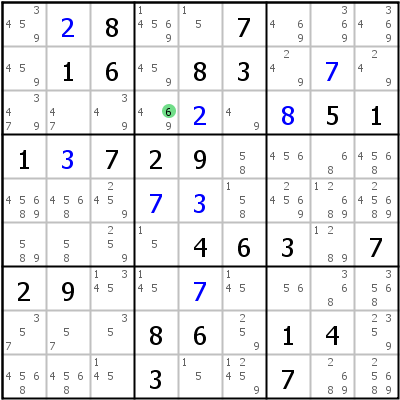
\includegraphics[scale=0.65]{figures/hidden_single.png} %以pic.jpg的0.5倍大小输出
\end{minipage}
}
\caption{Single Strategy} % %大图名称
\label{fig:1.5.2} %图片引用标记
\end{figure}

\subsubsection{Hidden Single}
Hidden Single means that for a given digit and house only one cell is left to place that digit. The cell itself has more than one candidate left, the correct digit is thus hidden amongst the rest.

\subsubsection{Naked Pair}
If you can find two cells, both in the same house, that have only the same two candidates left, you can eliminate that two candidates from all other cells in that house.

\subsubsection{Hidden Pair}
All Hidden Subsets work the same way, the only thing that changes is the number of cells and candidates affected by the move. Take Hidden Pair: If you can find two cells within a house such as that two candidates appear nowhere outside those cells in that house, those two candidates must be placed in the two cells. All other candidates can therefore be eliminated.

\begin{figure}[htbp]
\centering
\subfigure[Naked Pair]{
	\begin{minipage}{7cm}
	\centering
	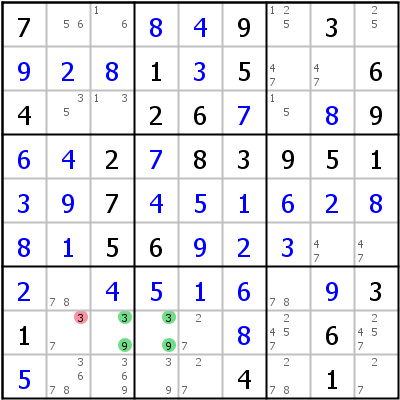
\includegraphics[scale = 0.65]{figures/naked_paire.png}
	\end{minipage}
}
\subfigure[Hidden Pair]{
	\begin{minipage}{7cm}
	\centering
	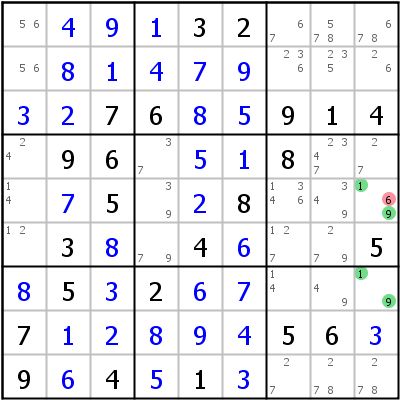
\includegraphics[scale = 0.65]{figures/hidden_pair.png}
	\end{minipage}
}
\caption{Pair Strategy}
\label{fig:1.5.3}
\end{figure}



\subsubsection{Hidden Triple}
Hidden Triples work in the same way as Hidden Pairs only with three cells and three candidates.\newline

All the strategies above will be used as the benchmark to test the difficulty of new-created sudoku puzzles.

\section{Analysis of the Problem}

\subsection{Model Building}


% \begin{figure}[ht]
% \small
% \centering
% 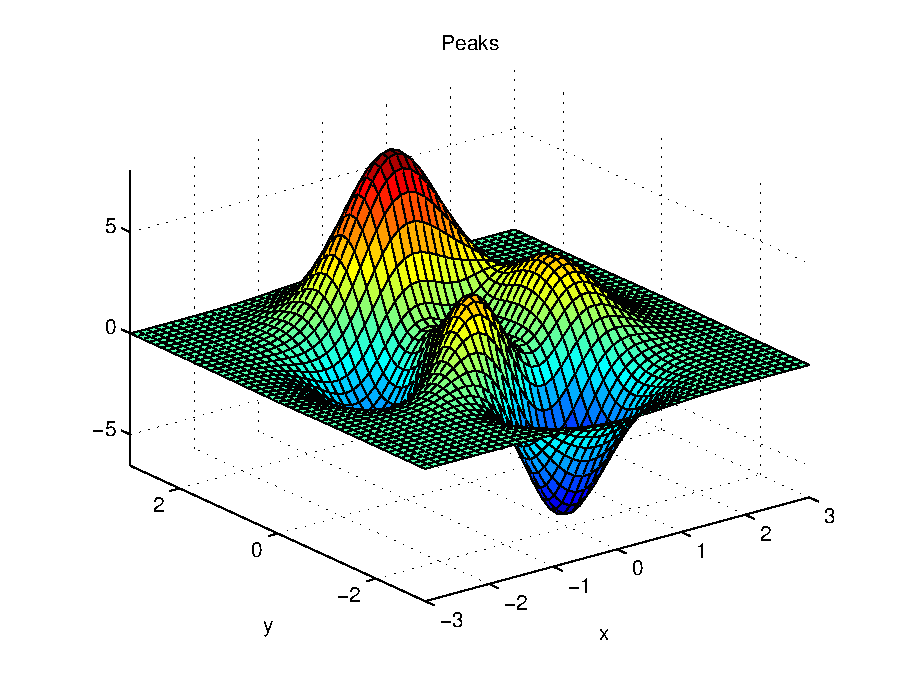
\includegraphics[width=12cm]{mcmthesis-aaa.eps}
% \caption{aa} \label{fig:aa}
% \end{figure}

% \lipsum[8] \eqref{aa}
% \begin{equation}
% a^2 \label{aa}
% \end{equation}

% \[
% \begin{pmatrix}{*{20}c}
% {a_{11} } & {a_{12} } & {a_{13} }  \\
% {a_{21} } & {a_{22} } & {a_{23} }  \\
% {a_{31} } & {a_{32} } & {a_{33} }  \\
% \end{pmatrix}
% = \frac{{Opposite}}{{Hypotenuse}}\cos ^{ - 1} \theta \arcsin \theta
% \]
% \lipsum[9]

% \[
% p_{j}=\begin{cases} 0,&\text{if $j$ is odd}\\
% r!\,(-1)^{j/2},&\text{if $j$ is even}
% \end{cases}
% \]

% \lipsum[10]

% \[
% \arcsin \theta  =
% \mathop{{\int\!\!\!\!\!\int\!\!\!\!\!\int}\mkern-31.2mu
% \bigodot}\limits_\varphi
% {\mathop {\lim }\limits_{x \to \infty } \frac{{n!}}{{r!\left( {n - r}
% \right)!}}} \eqno (1)
% \]

\section{Matrix Design}

\section{The Model Results}


\section{Evaluate of the Mode}
\subsection{Advantage of the Model}
\subsection{Disadvantage of the Model}

\section{Validating the Model}


\section{Conclusions}
in short but accurate

\section{A Summary}
\lipsum[6]


\section{Strengths and weaknesses}
\lipsum[12]

\subsection{Strengths}
\begin{itemize}
	\item \textbf{Applies widely}\\
	This  system can be used for many types of airplanes, and it also
	solves the interference during  the procedure of the boarding
	airplane,as described above we can get to the  optimization
	boarding time.We also know that all the service is automate.
	\item \textbf{Improve the quality of the airport service}\\
	Balancing the cost of the cost and the benefit, it will bring in
	more convenient  for airport and passengers.It also saves many
	human resources for the airline. \item \textbf{}
\end{itemize}

\begin{thebibliography}{99}
\bibitem{1} Donald E. Knuth: Dancing Links, Oxford-Microsoft Symposium on Computer Science, 2000
\bibitem{2}	Wikipedia: Sudoku
\bibitem{3}\url{http://blog.gssxgss.me/use-dlx-to-solve-sudoku-1/}
\end{thebibliography}

\begin{appendices}

\section{First appendix}

\lipsum[13]

Here are simulation programmes we used in our model as follow.\\

\textbf{\textcolor[rgb]{0.98,0.00,0.00}{Input matlab source:}}
\lstinputlisting[language=Matlab]{./code/mcmthesis-matlab1.m}

\section{Second appendix}

some more text \textcolor[rgb]{0.98,0.00,0.00}{\textbf{Input C++ source:}}
\lstinputlisting[language=C++]{./code/mcmthesis-sudoku.cpp}

\end{appendices}
\end{document}

%% 
%% This work consists of these files mcmthesis.dtx,
%%                                   figures/ and
%%                                   code/,
%% and the derived files             mcmthesis.cls,
%%                                   mcmthesis-demo.tex,
%%                                   README,
%%                                   LICENSE,
%%                                   mcmthesis.pdf and
%%                                   mcmthesis-demo.pdf.
%%
%% End of file `mcmthesis-demo.tex'.
